\documentclass[a4paper]{article}
\usepackage{latexsym}
\usepackage[a4paper]{geometry}
\usepackage{color}
\usepackage{listings}
\usepackage[pdftex]{graphicx}
\usepackage{float}
\usepackage{mathtools}
\usepackage{amsfonts, amsthm, amssymb}

\definecolor{Blue}{rgb}{0,0,0.5}
\definecolor{Green}{rgb}{0,0.75,0.0}
\definecolor{LightGray}{rgb}{0.6,0.6,0.6}
\definecolor{DarkGray}{rgb}{0.3,0.3,0.3}
\lstset{language=Matlab,
   keywords={function,uint8,uint16,uint32,double,break,case,catch,continue,else,elseif,end,for,global,if,otherwise,persistent,return,switch,try,while},
   basicstyle=\ttfamily\small,
   breaklines=true,
   keywordstyle=\bfseries\color{Blue},
   commentstyle=\itshape\color{LightGray},
   stringstyle=\color{Green},
   numbers=left,
   numberstyle=\tiny\color{DarkGray},
   stepnumber=1,
   numbersep=10pt,
   backgroundcolor=\color{white},
   tabsize=2,
   showspaces=false,
   showstringspaces=false,
   captionpos=b}

%Boldface text for type writer font
\usepackage{bold-extra} %\DeclareFontShape{OT1}{cmtt}{bx}{n}{<5><6><7><8><9><10><10.95><12><14.4><17.28><20.74><24.88>cmttb10}{}

%Break words properly at the end of a line (which isn't sloppy...)
\sloppy

%Use command \exercise for each exercise
\newcounter{exerciseCount}
\setcounter{exerciseCount}{0}
\newcommand{\exercise}[1]{\addtocounter{exerciseCount}{1} \noindent \medskip {\large \textsf{\textbf{Exercise \arabic{exerciseCount} \--- #1}}} \par}
\renewcommand{\theenumi}{\textsf{\textbf{\alph{enumi}}}}

%Use command \code for code snippets
\newcommand{\code}[1]{\textnormal{\texttt{#1}}}

\newtheorem*{claim}{Claim}
\renewcommand\qedsymbol{$\blacksquare$}

\title{\textsf{Image Processing \\ lab 4}}
\author{Klaas Kliffen \and Jan Kramer}
\date{\today}

\begin{document}
\maketitle

\exercise{Skeletons}
\noindent
The morphological skeleton of an image X with structuring element B is defined as:
\[
    SK(X) = \bigcup_{k = 0}^K S_{k}(X)
\]
where
\[
    S_{k}(X) = (X\ominus kB) - (X \ominus kB) \circ B
\]
and $K \in \mathbb{N}$ such that
\[
    K = max\{k |(X\ominus kB) \neq \emptyset\}.
\]
In addition $(X\ominus kB)$ is defined as follows:
\[
    (X \ominus kB) =
         \begin{cases}
             X      & \quad \text{if } k = 0\\
             ((\dots(X \ominus B) \ominus B) \ominus \dots) \ominus B) & \quad \text{otherwise} \\
         \end{cases}
\]
Note that in the second case $\ominus B$ is applied $k$ times to $X$.
\begin{enumerate}
\item
Let set $B = \hat{B} = \{0\}$ be given. \\
\begin{claim}
    $SK(X) = \emptyset$
\end{claim}
\begin{proof}
Note that for all $z \in \mathbb{Z}^{2}$ the following holds:
\[
    (B)_{z} = \{c|c = b + z, b \in B\} = \{c|c = z\} = \{z\}
\]
Then we have by the definition of the erosion of $X$ by $B$ that
\begin{align} \label{eq:ominus}
    X \ominus B &= \{z | (B)_{z} \subseteq X\} \nonumber\\
                &= \{z | \{z\} \subseteq X\} \\
                &= X. \nonumber
\end{align}
Similarly we have by the definition of the dilation of $X$ by $B$ that
\begin{align} \label{eq:oplus}
    X \oplus B &= \{z | (\hat{B})_{z} \cap X \neq \emptyset\} \nonumber\\
               &= \{z | \{z\} \cap X \neq \emptyset\} \\
               &= X. \nonumber
\end{align}
The skeleton of image $X$ with structuring element $B$ is:
\begin{align*}
    SK(X) &= \bigcup_{k = 0}^K S_{k}(X) \\
          &= \bigcup_{k = 0}^K \left((X\ominus kB) - (X \ominus kB) \circ B\right) \\
          &= \bigcup_{k = 0}^K \left((X \ominus kB) - ((X \ominus kB) \ominus B) \oplus B\right) \\
\end{align*}
Now if we apply the definition of $(X \ominus kB)$ and the results of equation \ref{eq:ominus} and \ref{eq:oplus} we get:
\begin{align*}
    SK(X) &= \bigcup_{k = 0}^K \left((X \ominus kB) - ((X \ominus kB) \ominus B) \oplus B\right) \\
          &= \bigcup_{k = 0}^K \left(X - X\right) \\
          &= \bigcup_{k = 0}^K \emptyset \\
          &= \emptyset
\end{align*}
\end{proof}

\item 
Let $X \ominus B = \emptyset$ be given.
\begin{claim}
    SK(X) = X
\end{claim}
\begin{proof}
Consider the definition of $(X \ominus kB)$:
\[
    (X \ominus kB) =
         \begin{cases}
             X      & \quad \text{if } k = 0\\
             ((\dots(X \ominus B) \ominus B) \ominus \dots) \ominus B) & \quad \text{otherwise} \\
         \end{cases}
\]
Note that $X \ominus B = \emptyset$. In addition for $X = \emptyset$ we have that every other erosion in the definition above is
\begin{equation} \label{eq:eominus}
    X \ominus B = \emptyset \ominus B = \{z | (B)_{z} \subseteq \emptyset\} = \emptyset.
\end{equation}
Hence the previous definition $X \ominus kB$ is equal to:
\begin{equation} \label{eq:kB}
    (X \ominus kB) =
         \begin{cases}
             X      & \quad \text{if } k = 0\\
             \emptyset & \quad \text{otherwise} \\
         \end{cases}
\end{equation}
Now the skeleton of image $X$ with structuring element $B$ is:
\begin{align*}
    SK(X) &= \bigcup_{k = 0}^K S_{k}(X) \\
          &= \bigcup_{k = 0}^K \left((X\ominus kB) - (X \ominus kB) \circ B\right) \\
          &= \bigcup_{k = 0}^K \left((X \ominus kB) - ((X \ominus kB) \ominus B) \oplus B\right) \\
          &= \left((X \ominus 0B) - ((X \ominus 0B) \ominus B) \oplus B\right) \cup \bigcup_{k = 1}^K \left((X \ominus kB) - ((X \ominus kB) \ominus B) \oplus B\right) \\
\end{align*}
If we use the equation \ref{eq:eominus}, \ref{eq:kB} and the definition of $X \oplus B$ we get:
\begin{align*}
    SK(X) &= \left(X - (X \ominus B) \oplus B\right) \cup \bigcup_{k = 1}^K \left(\emptyset - (\emptyset \ominus B) \oplus B\right) \\
          &= \left(X - (\emptyset \oplus B)\right) \cup \bigcup_{k = 1}^K \left(\emptyset - (\emptyset \oplus B)\right) \\
          &= \left(X - \{z | (\hat{B})_{z} \cap \emptyset \neq \emptyset\}\right) \cup \bigcup_{k = 1}^K \left(\emptyset - \{z | (\hat{B})_{z} \cap \emptyset \neq \emptyset\}\right) \\
          &= \left(X - \{z | \emptyset \neq \emptyset\}\right) \cup \bigcup_{k = 1}^K \left(\emptyset - \{z | \emptyset \neq \emptyset\}\right) \\
          &= \left(X - \emptyset \right) \cup \bigcup_{k = 1}^K \left(\emptyset - \emptyset\right) \\
          &= X \cup \bigcup_{k = 1}^K \emptyset \\
          &= X \cup \emptyset \\
          &= X 
\end{align*}
\end{proof}
\item
The implementation of IPskeletondecomp is rather trivial once one has the basic morphologic functions implemented.
The only non-trivial thing is the subtraction in $S_k(X)$.
Since the second term is always smaller than the first one, because of the extra erosion, the xor function can be used to get the difference.
Then it is just implementing the definition:
\lstinputlisting{../lab4ex1/IPskeletondecomp.m}
The implementation of dilation is also rather simple, because the 2 dimensional convolution function can be used:
\lstinputlisting{../lab4ex1/IPdilate.m}
The implementation of erosion can than be based on the one of dilation, because of their duality.
Note however that the image has to be padded so that this works:
\lstinputlisting{../lab4ex1/IPerode.m}
\item
Basically the reconstruction works by taking the union of dilating the skeleton parts the correct amount.
This can be done as follows:
\lstinputlisting{../lab4ex1/IPskeletonrecon.m}
\item
To demonstrate that the decomposition and the reconstruction works, we wrote the following script to compare the results:
\lstinputlisting{../lab4ex1/runex1.m}
The result of running this script is as follows:
\begin{lstlisting}
ans = 0.
\end{lstlisting}
This means that the original and the resulting image are identical.
In addition these images can be seen in Figure \ref{fig:nutsbolts}.
\begin{figure}[H]
\centering
\begin{tabular}{ccc}
    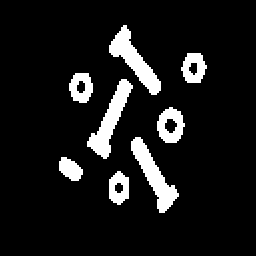
\includegraphics[width=0.3\textwidth]{../lab4ex1/nutsbolts.png} & 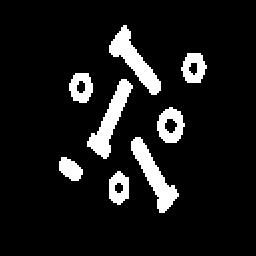
\includegraphics[width=0.3\textwidth]{../lab4ex1/recon.png}  & \\
    Original image & The result of decomposition and reconstruction \\
\end{tabular}
\caption{The nutsbolts image and its skeleton decomposition reconstruction.}
\label{fig:nutsbolts}
\end{figure}
\end{enumerate}


\exercise{Grey-scale morphology}
\begin{enumerate}
\item
Based on the equation 9.2-1 in the book, the implementation of IPgerode is rather straightforward:
\lstinputlisting{../lab4ex2/IPgdilate.m}
The only trick used here is to use the NaN value to ignore pixels that are outside the picture or not part of the structuring element.
This works because $min(NaN, 3) = 3$ and $max(NaN, 3) = 3$.
The only problem is that $NaN$ does not exist for uint8's, therefore the image has to be converted to double before the calculations and back afterwards.
Also note that maximum/minimum of the elements of the matrices is calculated by taking the the pairwise maxima/minima.
The implementation of IPgdilate is based on equation 9.2-2 in the book and the implementation of IPgerode:
\lstinputlisting{../lab4ex2/IPgerode.m}
\item
The resulting images are shown in figure \ref{fig:gray}.
Like mentioned in example 9.9 of the book the erosion increases the size and intensity of dark features, while decreasing the bright ones.
For example the branches of the plant are darker and bigger, while the water in the vase is less bright.
This is the result of the minimum operation in the definition of gray-scale erosion.
Similarly that example in the dilation bright features are increased in size and intensity, while decreasing the size and intensity of dark features.
In this case the branches are thinner and smaller than in the original and the water in the vase is brighter.
Also note that smaller features may be more visible by erosion or dilation depending on if they are dark respectively bright.
In addition example 9.10 in the book discusses gray-scale openings and closings.
The opening decreases the intensity of bright features smaller than the structuring element, while keeping the dark ones relative the same.
Note for example the decreased intensity of the spots in the vase.
The closing decreased the intensity of dark features smaller than the structuring element, while keeping the bright ones.
Again the dots in the vase show this.
\begin{figure}[H]
\centering
\begin{tabular}{ccc}
    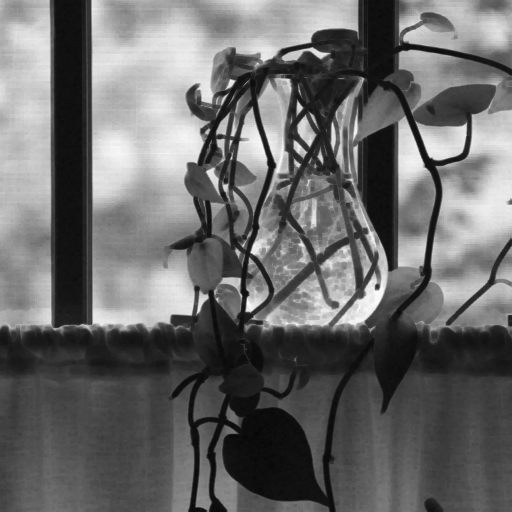
\includegraphics[width=0.3\textwidth]{../lab4ex2/gerode.png} & 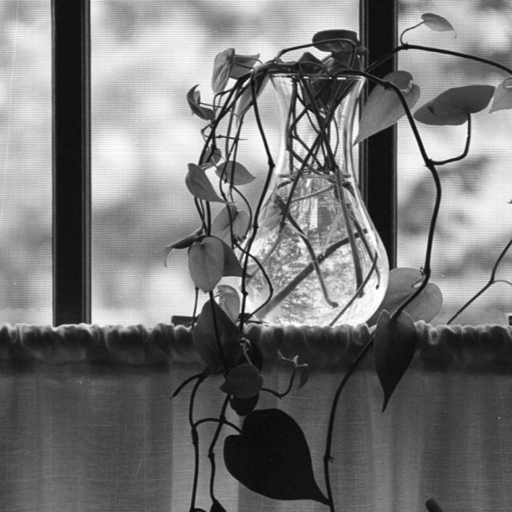
\includegraphics[width=0.3\textwidth]{../lab4ex2/vase.png} & 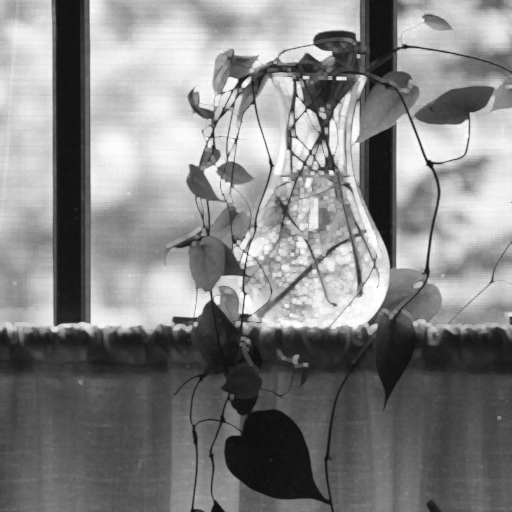
\includegraphics[width=0.3\textwidth]{../lab4ex2/gdilate.png} \\
    The erosion & Original image & The dilation \\
    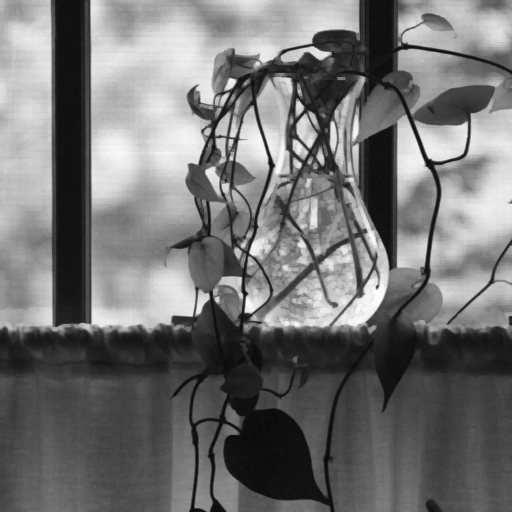
\includegraphics[width=0.3\textwidth]{../lab4ex2/gopening.png} & 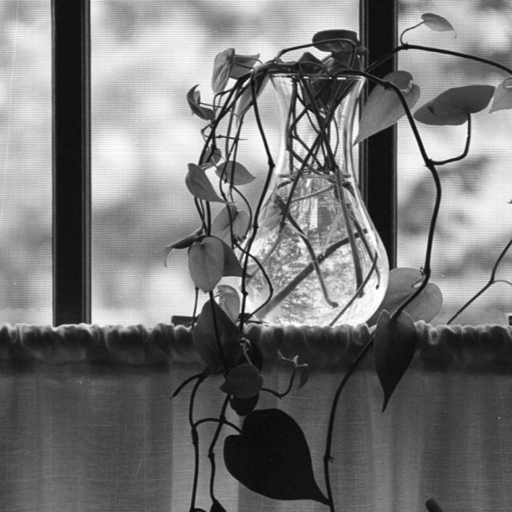
\includegraphics[width=0.3\textwidth]{../lab4ex2/vase.png} & 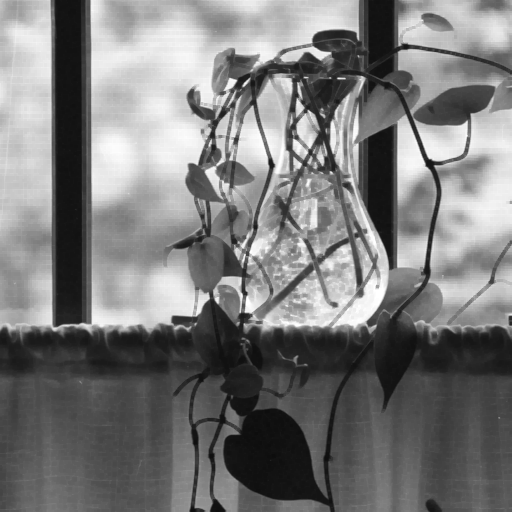
\includegraphics[width=0.3\textwidth]{../lab4ex2/gclosing.png} \\
    The opening & Original image & The closing \\
\end{tabular}
\caption{The grayscale dilation, erosion, opening and closing of vase.tif with a flat box structuring element.}
\label{fig:gray}
\end{figure}

\end{enumerate}

\exercise{Classification}

\noindent suppress the small disks in the image, they need to be eroded.
By choosing a structuring element larger than the small disks, only the large disks will be left.
However, the large disks are eroded and need to be reconstructed.
This can be done by dilating the eroded image with a similar structuring element.
To fully reconstruct the old disks, the original image and the dilated image can be considered a set.
By taking the union of these two sets, the large disks will be restored, while the small disks will disappear.
Since the possible overflow of the dilated image will be suppressed by the original image and the small disks are suppressed by the 
dilated image.\\

\noindent To be able to use set operations, the image is first converted to binary image with a foreground and background by a certain threshold.
This will also suppress all noise in the image and only the disks will be shown as can be seen in figure \ref{fig:binarymask}.
\lstinputlisting{../lab4ex3/makebinary.m}

\begin{figure}[H]
\centering
\begin{tabular}{cc}
    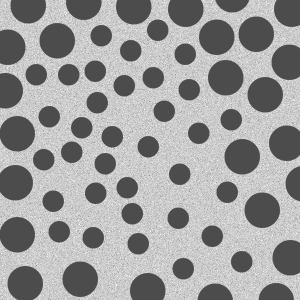
\includegraphics[width=0.3\textwidth]{../lab4ex3/blobs.png} & 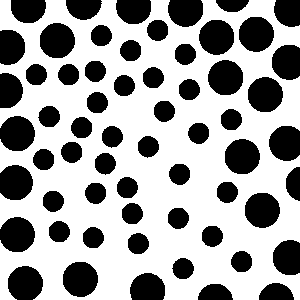
\includegraphics[width=0.3\textwidth]{../lab4ex3/binarymask.png} \\
    The original image & The binary thresholded image\\
\end{tabular}    
    
\caption{The original image is being converted to a binary image}
\label{fig:binarymask}
\end{figure}

\noindent To suppress the small disks an erosion is used. This is implemented by using a 2D convolution with the structuring element.
This element is generated by creating a square matrix of ones and a circular element of zeros with a given radius.
Zeros are being used, since the disks are also considered background.
Since both images are binary, this will be the same as performing the opening operation. The result of the 
convolution can be seen in figure \ref{fig:convolution}. The small disks have been removed by the convolution.

\begin{figure}[H]
  \centering
  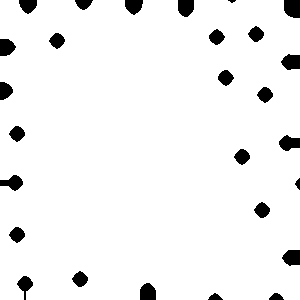
\includegraphics[width=0.3\textwidth]{../lab4ex3/convolution.png} 
  \caption{The erosion convolution of figure \ref{fig:binarymask} with a circular structuring element of radius 8}
  \label{fig:convolution}
\end{figure}



\lstinputlisting{../lab4ex3/makeblob.m}

\newpage

\noindent Next the large disks have to be reconstructed.
This is done by eroding the background instead of the foreground.
Therefor the complement of figure \ref{fig:convolution} is taken for the next convolution step.
A large structuring element is chosen, so to be sure that all pixels from the large disks in figure \ref{fig:binarymask} are covered.
Normally the and operation would be used to restore the final images, but since both images are actually the complement since
the disks consist of 0 values, the or operation is used.
This is derived by using De Morgan's laws for converting the and of two negated operand to the or operation.\\

\noindent Furthermore, using a too large structuring element will restore some parts of the small disks.
Therefor the dilation is done in two steps: one with a circular structuring with radius 11 and one with radius 4.
The resulting image can be seen in figure \ref{fig:restored}.

\begin{figure}[H]
  \centering
  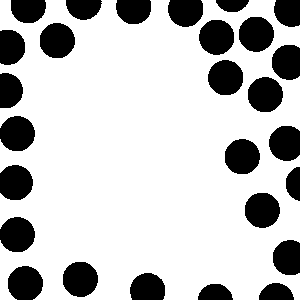
\includegraphics[width=0.3\textwidth]{../lab4ex3/restored.png} 
  \caption{The dilation convolution of figure \ref{fig:convolution} with a circular structuring element of radius 11 and 4}
  \label{fig:restored}
\end{figure}

\noindent To fully restore the original values of the large disks, the complement of figure \ref{fig:restored} is element wise multiplied by the original image as seen 
on the left of figure \ref{fig:binarymask}. This will remove all the small disks, but also the noisy background.
To somewhat represent the contrast of the original image, the mean value of the noise is used as the background which was deleted by thresholding
in the first step. The final image can be seen in figure \ref{fig:final}

\begin{figure}[H]
\centering
\begin{tabular}{cc}
    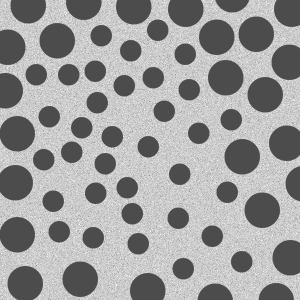
\includegraphics[width=0.3\textwidth]{../lab4ex3/blobs.png} & 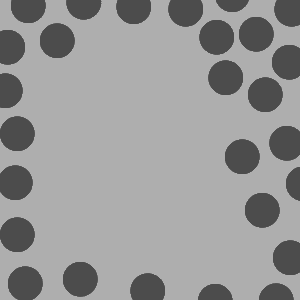
\includegraphics[width=0.3\textwidth]{../lab4ex3/final.png} \\
    The original image & The final image with the small disks and noise removed\\
\end{tabular}    
    
\caption{A comparison of the original image with the final image}
\label{fig:final}
\end{figure}


\newpage

\lstinputlisting{../lab4ex3/runex3.m}~\\
\noindent The downside of using this method, is that the mask used is binary. Therefor, the edges of
the large disks are quite sharp. This can be solved by applying a weak blurring filter.
Also, the removed noise might be considered a downside of this method, since the visual contrast
of the image is decreased. However, for computer vision application such as feature detection
it might be a benefit.

\newpage
\section*{Task distribution}

\begin{table}[H]
\centering
\begin{tabular}{ccccc}
ex1 & design & implementation & answers questions & writing report \\
\hline
Klaas & 20\% & 10\% & 20\% & 40\% \\
\hline
Jan & 80\% & 90\% & 80\5 & 60\% \\
\end{tabular}
\end{table}

\begin{table}[H]
\centering
\begin{tabular}{ccccc}
ex2 & design & implementation & answers questions & writing report \\
\hline
Klaas & 50\% & 20\% & 25\% & 25\% \\
\hline
Jan & 50\% & 80\% & 75\% & 75\% \\
\end{tabular}
\end{table}

\begin{table}[H]
\centering
\begin{tabular}{ccccc}
ex3 & design & implementation & answers questions & writing report \\
\hline
Klaas & 80\% & 75\% & 75\% & 80\% \\
\hline
Jan & 20\% & 25\% & 25\% & 20\% \\
\end{tabular}
\end{table} 



\end{document}
